
\documentclass{bredelebeamer}


\usepackage{amsmath}

\usepackage{algorithmicx}
\usepackage{algpseudocode}
\usepackage{parcolumns}
\usepackage{lipsum}

\usepackage{listings}

\lstdefinestyle{CStyle}{
    backgroundcolor=\color{backgroundColour},
    commentstyle=\color{mGreen},
    keywordstyle=\color{magenta},
    numberstyle=\tiny\color{mGray},
    stringstyle=\color{mPurple},
    basicstyle=\scriptsize,
    %basicstyle=\tiny,
    breakatwhitespace=false,
    breaklines=true,
    captionpos=t,
    keepspaces=true,
    numbers=left,
    numbersep=5pt,
    showspaces=false,
    showstringspaces=false,
    showtabs=false,
    tabsize=2,
    language=C
}

\lstdefinestyle{customasm}{
  belowcaptionskip=1\baselineskip,
  frame=L,
  xleftmargin=\parindent,
  language=[x86masm]Assembler,
  basicstyle=\footnotesize\ttfamily,
  commentstyle=\itshape\color{purple!40!black},
}

\usepackage{placeins}

\usepackage{parskip}
%%%%%%%%%%%%%%%%%%%%%%%%%%%%%%%%%%%%%%%%%%%%%%%%



\title[Calcul du flux optique sur Raspbery Pi]{Implémentation embarquée d'un algorithme de calcul de flux optique sur un dr\^one sous-marin autonome}
% Titre du diaporama

\subtitle{Processeur Graphique \textsc{VideoCore IV 3D}}
% Sous-titre optionnel

\author{Simon Bataille\inst{1}}
% La commande \inst{...} Permet d'afficher l' affiliation de l'intervenant.
% Si il y a plusieurs intervenants: Marcel Dupont\inst{1}, Roger Durand\inst{2}
% Il suffit alors d'ajouter un autre institut sur le modèle ci-dessous.

\institute[Université de Caen Normandie]
{
  \inst{1}%
  ESIX NORMANDIE\\
  Département Mécatronique \& Systèmes Nomades
  }


\date{28 Septembre 2018}
% Optionnel. La date, généralement celle du jour de la conférence

\subject{Stage de fin d'étude}
% C'est utilisé dans les métadonnes du PDF



\logo{

\includegraphics[scale=0.3]{images/logoNotilo.png}
}



%%%%%%%%%%%%%%%%%%%%%%%%%%%%%%%%%%%%%%%%%%%%%%%%%%%%%%%%%%%%%%%%%%%%%
\begin{document}

\begin{frame}
  \titlepage
\end{frame}





\begin{frame}{Sommaire}
  \tableofcontents
  % possibilité d'ajouter l'option [pausesections]
\end{frame}




%%%%%%%%%%%%%%%%%%%%%%%%%%%%%%%%%%%%%%%%%%%%%%%%%%%%%%%%%%%%%%%%%%%%%
%%%%%%%%%%%%%%%%%%%%%%%%%%%%%%%%%%%%%%%%%%%%%%%%%%%%%%%%%%%%%%%%%%%%%

\section{Introduction}

%%%%%%%%%%%%%%%%%%%%%%%%%%%%%%%%%%%%%%%%%%%%%%%%%%%%%%%%%%%%%%%%%%%%%

	\subsection{Notilo+}

%-----------------------------------------------------------------------------

\begin{frame}{Notilo+}

\begin{block}{Entreprise d'accueil}
\begin{itemize}
\item Jeune start-up créée à Lyon en 2016
\item Développement d'un dr\^one sous-marin autonome: iBubble
\begin{figure}
\centering
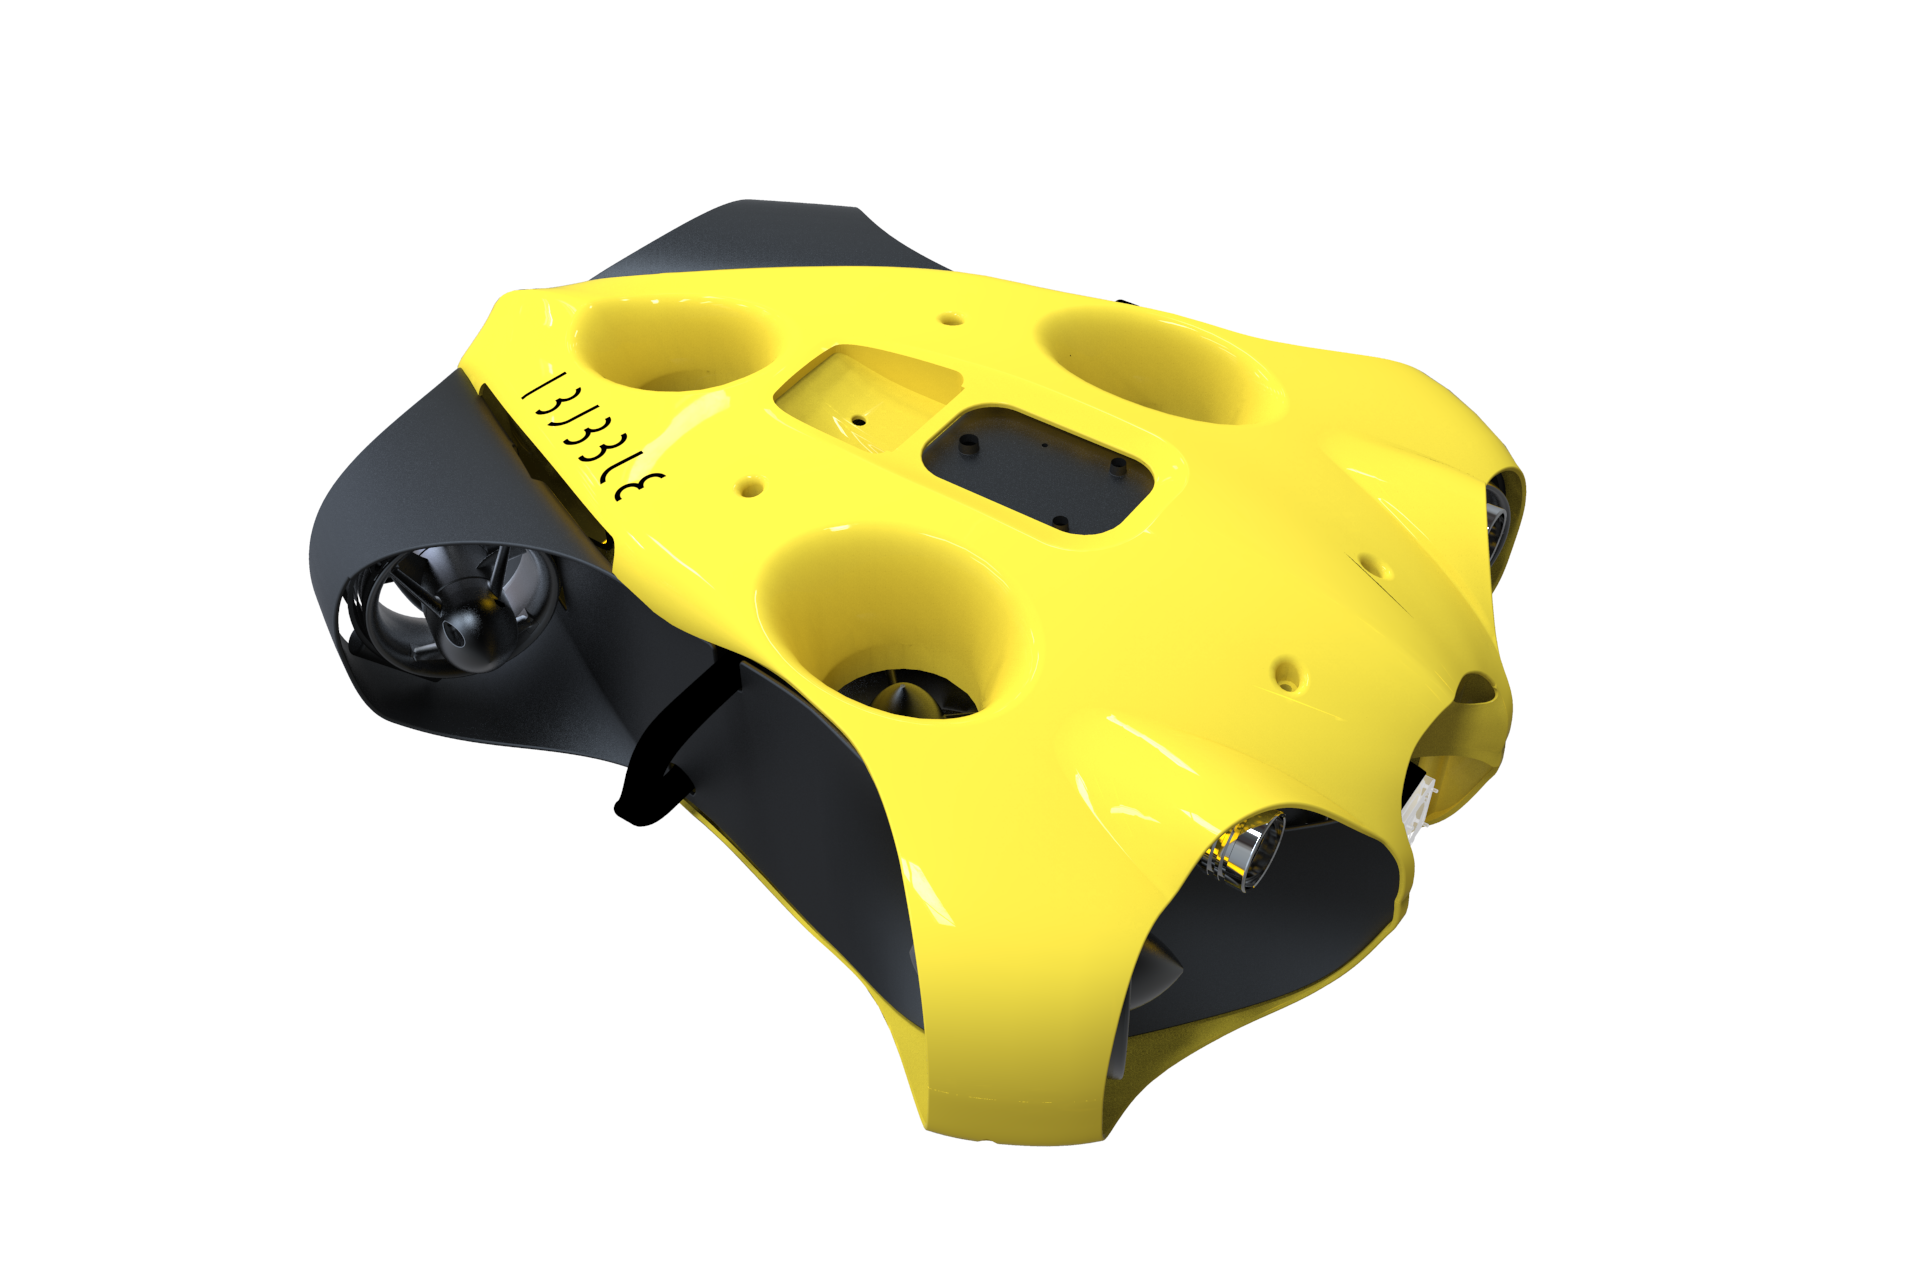
\includegraphics[scale=0.05]{images/iBubble3.png}
\caption{iBubble}
\end{figure}
\item Environ 25 personnes réparties en 2 équipes:
	\begin{itemize}
	\item équipe commerciale
	\item équipe technique
	\end{itemize}
\item Tuteur: Filip Novotny -- responsable de la partie vision
\item Thibault Anquetil -- ancien élève à l'ESIX
\end{itemize}
\end{block}

\end{frame}

%-----------------------------------------------------------------------------



%%%%%%%%%%%%%%%%%%%%%%%%%%%%%%%%%%%%%%%%%%%%%%%%%%%%%%%%%%%%%%%%%%%%%

	\subsection{iBubble}

%-----------------------------------------------------------------------------

\begin{frame}{iBubble}

\begin{block}{Caractéristiques}
\begin{itemize}
\item Aquatique et Autonome
\item Repérage Acoustique
\item Système de Suivi Visuel
\end{itemize}
\end{block}

\begin{block}{Développement}
\begin{itemize}
\item Hardware: mécanique et conception électronique
\item Embarquée: logiciel pilotant iBubble
\item Informatique haut niveau: algorithmes de suivi par vision
\end{itemize}
\end{block}

\end{frame}

%-----------------------------------------------------------------------------




%%%%%%%%%%%%%%%%%%%%%%%%%%%%%%%%%%%%%%%%%%%%%%%%%%%%%%%%%%%%%%%%%%%%%

	\subsection{Problématique}

%-----------------------------------------------------------------------------

\begin{frame}{Problématique}

\begin{block}{Algorithme de tracking visuel}
\begin{itemize}
\item CMT -- algorithme de suivi visuel bien connu
\item Initialement, iBubble développé avec une carte Jetson
\begin{itemize}
\item GPGPU à architecture CUDA
\item Optimisation du CMT à 30 images par seconde
\end{itemize}
\end{itemize}
\end{block}

\begin{block}{Raspberry Pi}
\begin{itemize}
\item Carte embarquée sur la version commerciale de iBubble
\item SoC BCM2837 -- BROADCOM
\begin{itemize}
\item CPU -- ARM
\item GPU VideoCore IV 3D -- BROADCOM
\end{itemize}
\item Pas une architecture CUDA
\begin{itemize}
	\item Pas d'optimation du CMT
	\item VideoCore inutilisé
	\item 7 images par seconde
\end{itemize}
\end{itemize}
\end{block}

\end{frame}

%-----------------------------------------------------------------------------



%%%%%%%%%%%%%%%%%%%%%%%%%%%%%%%%%%%%%%%%%%%%%%%%%%%%%%%%%%%%%%%%%%%%%

	\subsection{Réponse}

%-----------------------------------------------------------------------------

\begin{frame}{Réponse}
\begin{block}{Flux optique}
\begin{itemize}
\item Calcul du Flux Optique
\begin{itemize}
	\item Partie du CMT qui consomme le plus de ressources
	\item Parallèlisable sur GPU
\end{itemize}
\item Implémentation interne du calcul du Flux Optique
\item Utilisation du GPU de la Rasperry Pi pour certains calculs
\end{itemize}
\end{block}

\begin{exampleblock}{Tâches}
\begin{itemize}
\item Comprendre l'archtecture du VideoCore IV 3D
\item Apprendre à programmer le VideoCore IV 3D
\item Implémenter le calcul du Flux Optique sur Raspberry Pi
\end{itemize}
\end{exampleblock}

\begin{alertblock}{Difficultés}
\begin{itemize}
\item Aucune API officielle éxistante pour l'utilisation du VideoCore IV 3D
\item Programmation en assembleur à partir de projets non-officiels
\end{itemize}
\end{alertblock}

\end{frame}

%-----------------------------------------------------------------------------



%%%%%%%%%%%%%%%%%%%%%%%%%%%%%%%%%%%%%%%%%%%%%%%%%%%%%%%%%%%%%%%%%%%%%
%%%%%%%%%%%%%%%%%%%%%%%%%%%%%%%%%%%%%%%%%%%%%%%%%%%%%%%%%%%%%%%%%%%%%

\section{Sujet}

%%%%%%%%%%%%%%%%%%%%%%%%%%%%%%%%%%%%%%%%%%%%%%%%%%%%%%%%%%%%%%%%%%%%%

	\subsection{Flux Optique}


%-----------------------------------------------------------------------------

\begin{frame}{Données entrantes: que traite-t-on ?}


\begin{block}{Images issues de la RaspiCam}
\begin{itemize}
\item Matrices $240\times 360$ -- floats 32-bit $\in \left[0;1\right]$
\item Lignes contigues en RAM -- Row-major
\item Adressage 32-bit
\end{itemize}
\end{block}

\begin{figure}
\centering
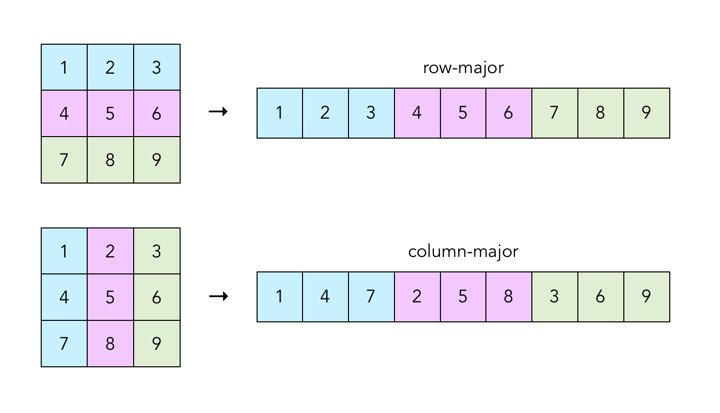
\includegraphics[scale=0.2]{images/rowcolumnarrays.jpg}
\caption{Stockage des pixels en RAM}
\end{figure}


\end{frame}

%-----------------------------------------------------------------------------

\begin{frame}{Données entrantes: que traite-t-on ?}


\begin{block}{Features}
\begin{itemize}
\item Points d'intér\^ets encadrants le plongeur
\item Utiliser dans le CMT pour suivre le plongeur
\item Repérées par le couple $(x,y)$:
	\begin{itemize}
		\item $x$ -- ligne de la feature $\in \left[0;240\right]$
		\item $y$ -- colonne de la feature $\in \left[0;360\right]$
	\end{itemize}
\end{itemize}
\end{block}

\begin{figure}
\centering
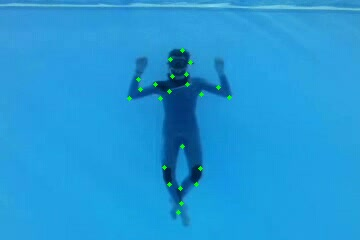
\includegraphics[scale=0.5]{images/plongeurInitFeatures.jpeg}
\end{figure}


\end{frame}

%-----------------------------------------------------------------------------

\begin{frame}{Flux Optique}

\begin{alertblock}{Flux Optique}
Déplacement de ces features entre 2 images consécutives d'une vidéo
\begin{itemize}
	\item $d_{x}$: déplacement de la feature suivant les lignes
	\item $d_{y}$: déplacement de la feature suivant les colonnes
	\item Déplacements mesurés en pixels
\end{itemize}
\end{alertblock}

\begin{figure}
\centering
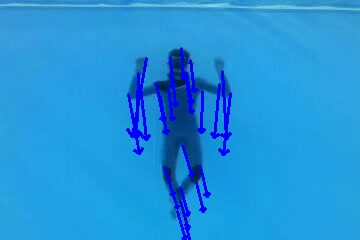
\includegraphics[scale=0.4]{images/plongeurOpticalFlow.jpeg}
\caption{Flux optique entre les 2 images}
\end{figure}

\end{frame}

%-----------------------------------------------------------------------------

\begin{frame}{Flux Optique entre 2 images successives}

\begin{columns}

\begin{column}{0.3\textwidth}
\begin{figure}
\centering
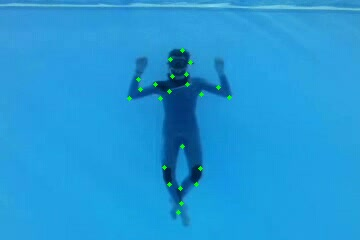
\includegraphics[scale=0.3]{images/plongeurInitFeatures.jpeg}
\caption{FEATURES sur la première image}
\end{figure}
\end{column}


\begin{column}{0.3\textwidth}
\begin{figure}
\centering
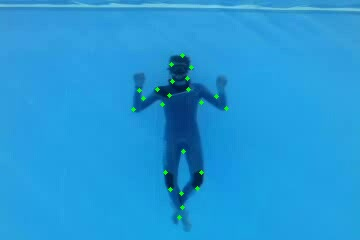
\includegraphics[scale=0.3]{images/plongeurNextFeatures.jpeg}
\caption{FEATURES sur la deuxième image}
\end{figure}
\end{column}

\end{columns}

%\begin{column}{0.3\textwidth}
\begin{figure}
\centering
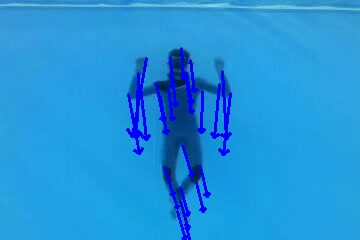
\includegraphics[scale=0.3]{images/plongeurOpticalFlow.jpeg}
\caption{Flux optique entre les 2 images}
\end{figure}
%\end{column}

%\end{columns}

\end{frame}

%-----------------------------------------------------------------------------

\begin{frame}{Flux Optique d'une seule FEATURE entre 2 images successives}

\begin{figure}
%\centering
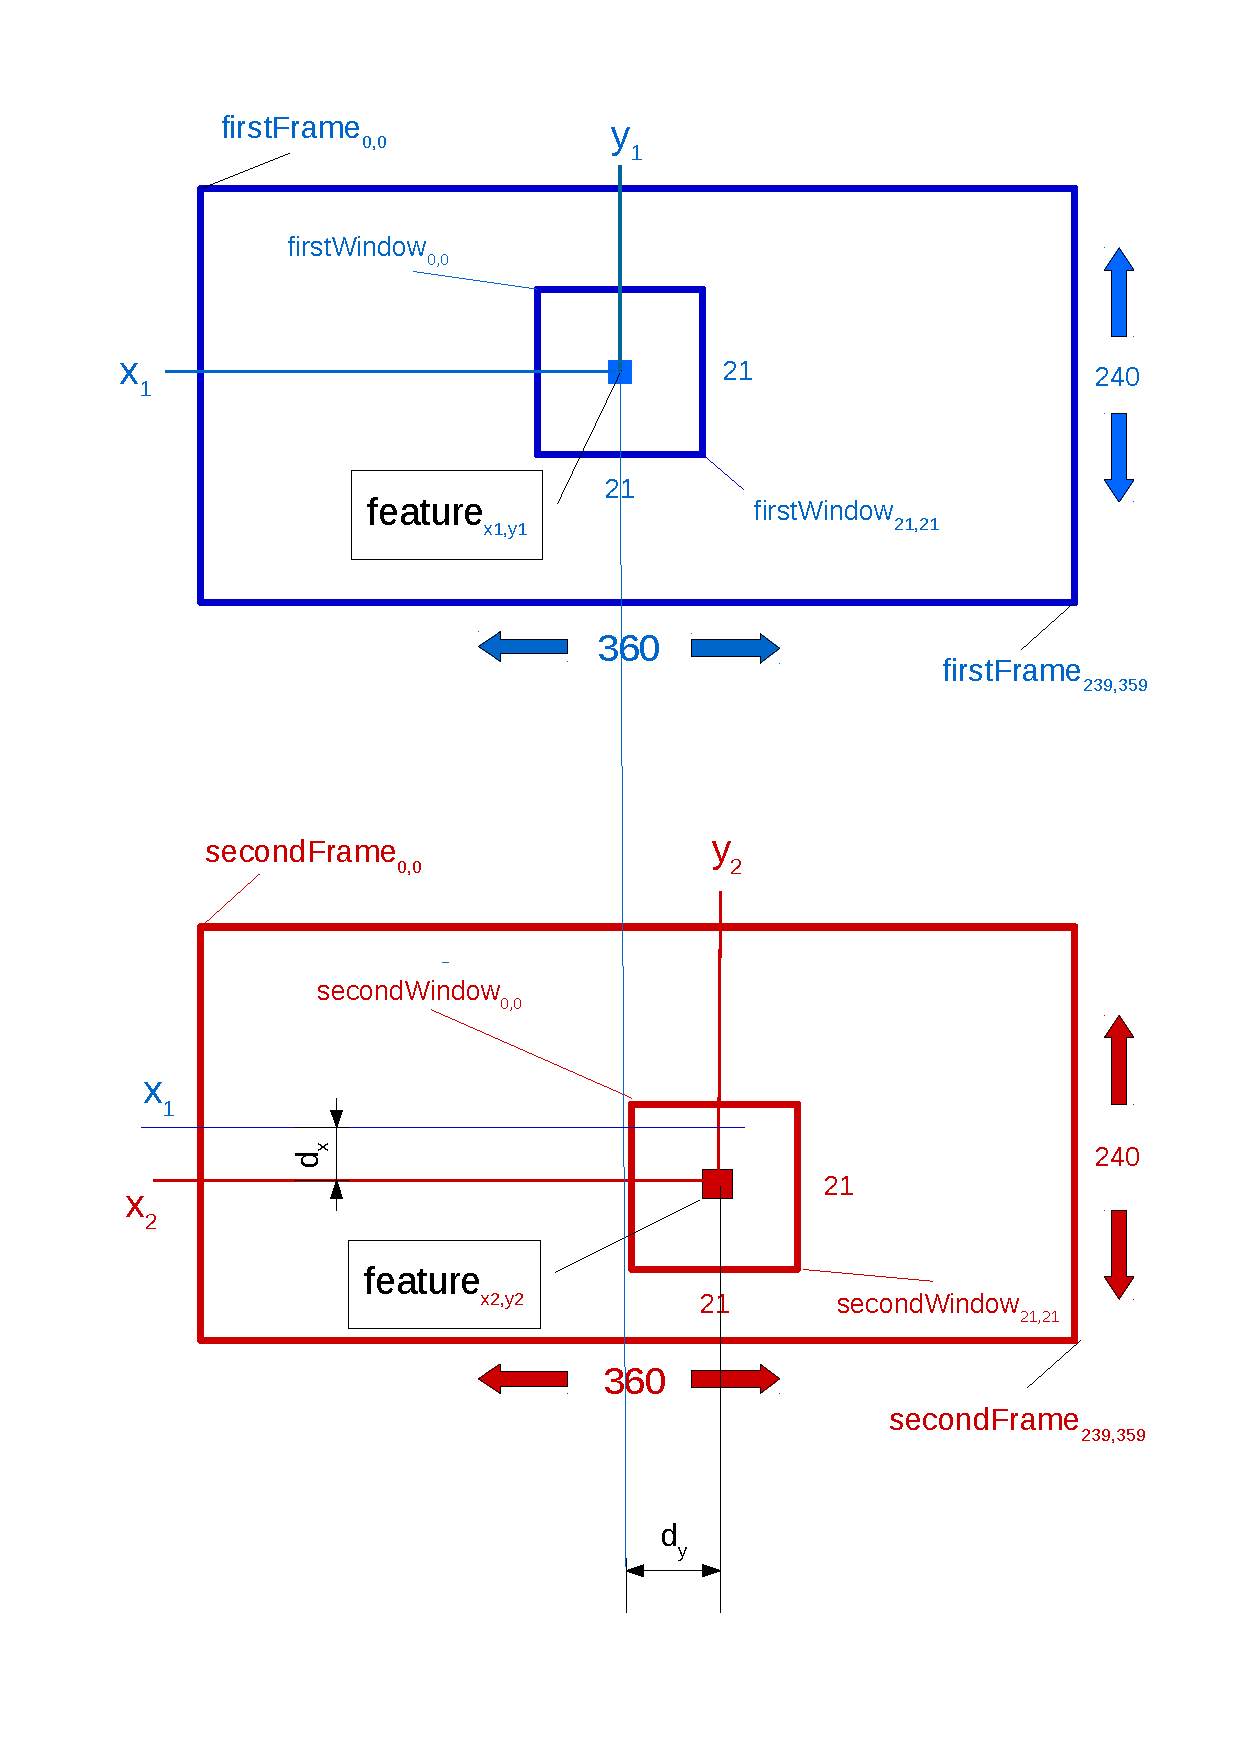
\includegraphics[scale=0.3]{images/framesWindow.pdf}
\end{figure}

\end{frame}

%-----------------------------------------------------------------------------

%%%%%%%%%%%%%%%%%%%%%%%%%%%%%%%%%%%%%%%%%%%%%%%%%%%%%%%%%%%%%%%%%%%%%
	\subsection{Méthode de Lucas-Kanade}

%-----------------------------------------------------------------------------

\begin{frame}{Méthode de Lucas-Kanade}

\begin{block}{Estimation du Flux Optique pour chaque FEATURE}
\begin{itemize}
	\item Plusieurs algorithmes permettant le calcul
	\item Camille a sélectionné la Méthode de Lucas-Kanade -- Algorithme bien connu
	\item Entre 2 images successives
\end{itemize}
\end{block}

\begin{exampleblock}{2 Etapes}
\begin{itemize}
	\item Première étape dite de Gradient sur la première image
	\item Deuxième étape du calcul effectif du fluxa optique pour chaque FEATURE
	\item 30 FEATURES sur l'image -- 1 seule FEATURE
\end{itemize}
\end{exampleblock}

\end{frame}

%-----------------------------------------------------------------------------

\begin{frame}{Gradient sur la première image pour une FEATURE}

	\begin{block}{4 Valeurs à calculer}
\begin{itemize}
	\item $G_{XX}$ -- gradient vertical de la FEATURE
	\item $G_{YY}$ -- gradient horizontal de la FEATURE
	\item $G_{XY}$ -- gradient croisé de la FEATURE
	\item $det = \frac{1}{G_{XX}G_{YY}-G_{XY}G_{XX}}$
\end{itemize}
\end{block}


\boitejaune{
	$$G_{YY} = \sum_{i=1}^{21}\sum_{j=1}^{21} grad_{y}[i,j]^{2}$$\\
	$$G_{XY} = \sum_{i=1}^{21}\sum_{j=1}^{21} grad_{x}[i,j]\times grad_{y}[i,j]$$\\
	$$G_{XX} = \sum_{i=1}^{21}\sum_{j=1}^{21} grad_{x}[i,j]^{2}$$
}

\end{frame}

%-----------------------------------------------------------------------------

\begin{frame}{Gradient sur la première image pour une FEATURE}

	\begin{block}{Fen\^etre autour de la FEATURE}
 $$grad_{x}[i,j] = \frac{\textcolor{blue}{firstWindow_{i+1,j}} - \textcolor{blue}{firstWindow_{i-1,j}}}{2}$$
 $$grad_{y}[i,j] = \frac{\textcolor{blue}{firstWindow_{i,j+1}} - \textcolor{blue}{firstWindow_{i,j-1}}}{2}$$
\end{block}

\begin{figure}
%\centering
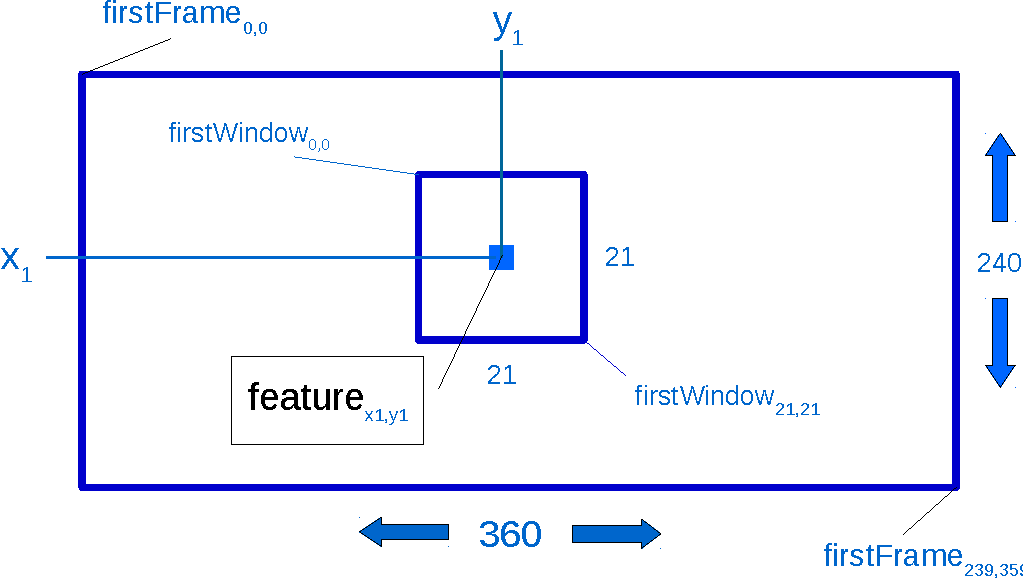
\includegraphics[scale=0.3]{images/firstFrameWindow.pdf}
\end{figure}

\end{frame}

%-----------------------------------------------------------------------------

\begin{frame}{Flux Optique: $d_{x}, d_{y}$}

	\begin{block}{Algorithme de calcul du déplacement}
\begin{algorithmic}
	\ForAll {$\textcolor{blue}{firstWindow_{i,j}}$ and $\textcolor{red}{secondWindow_{i,j}}$}

	\State $diff\_frames = \textcolor{blue}{firstWindow_{i,j}} - \textcolor{red}{secondWindow_{i+d_{x},j+d_{y}}}$

	\State $frames\_mismatch.x = diff\_frames\times grad_{x}[i,j]$
	\State $frames\_mismatch.y = diff\_frames\times grad_{y}[i,j]$

	\EndFor

	\State $d_{x} = det\times (G_{YY}\times frames\_mismatch.x - G_{XY}\times frames\_mismatch.y)$
	\State $d_{y} = det\times (G_{XX}\times frames\_mismatch.y - G_{XY}\times frames\_mismatch.x)$
\end{algorithmic}
\end{block}

	\begin{alertblock}{Interpolation Bilinéaire}
\begin{equation*}
	\begin{split}
		\textcolor{red}{secondWindow_{i+d_{x},j+d_{y}}} =\\
		\textcolor{red}{secondWindow_{floor(i+d_{x}),floor(j+d_{y})}}\times (1-fract(i+d_{x}))\times (1-fract(i+d_{y}))\\
		+ \textcolor{red}{secondWindow_{floor(i+d_{x})+1,floor(j+d_{y})}}\times (fract(i+d_{x}))\times (1-fract(i+d_{y}))\\
		+ \textcolor{red}{secondWindow_{floor(i+d_{x}),floor(j+d_{y})+1}}\times (1-fract(i+d_{x}))\times (fract(i+d_{y}))\\
		+ \textcolor{red}{secondWindow_{floor(i+d_{x})+1,floor(j+d_{y})+1}}\times (fract(i+d_{x}))\times (fract(i+d_{x}))
	\end{split}
\end{equation*}
	\end{alertblock}

\end{frame}

%-----------------------------------------------------------------------------

\begin{frame}{Flux Optique d'une seule FEATURE entre 2 images successives}

\begin{figure}
%\centering
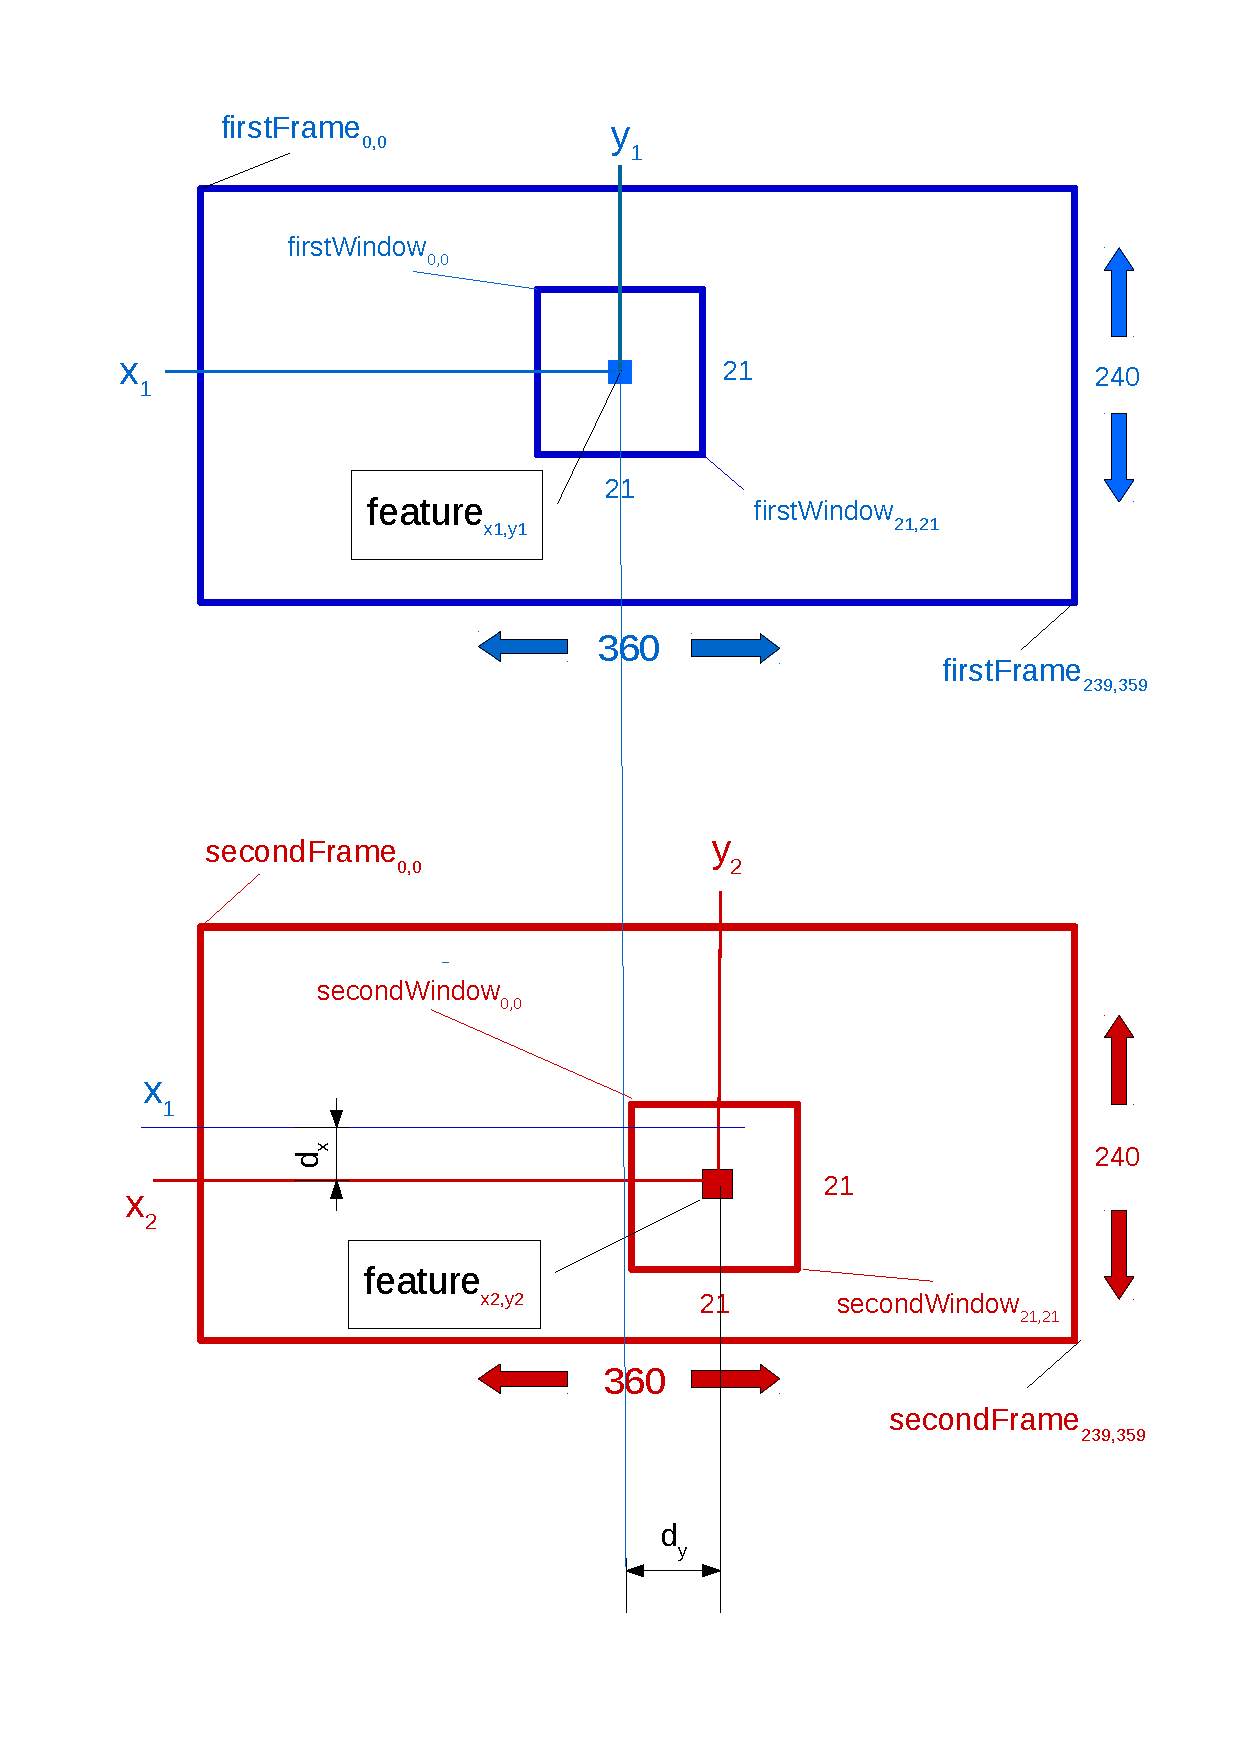
\includegraphics[scale=0.3]{images/framesWindow.pdf}
\end{figure}

\end{frame}

%-----------------------------------------------------------------------------

%%%%%%%%%%%%%%%%%%%%%%%%%%%%%%%%%%%%%%%%%%%%%%%%%%%%%%%%%%%%%%%%%%%%%
	\subsection{VideoCore IV 3D}
\begin{frame}{Architecture}
\begin{block}{Bloc simple}
\begin{itemize}
\item Documentation Officielle
\item Aucune API officielle
\item Jeu d'instructions
\item Vecteurs de 16 mots
\end{itemize}
\end{block}

\end{frame}

\begin{frame}{Programmation}
\begin{block}{Bloc simple}
\begin{itemize}
\item Piloter par un CPU: interface mailbox
\item Mémoire RAM partagée entre CPU \& GPU: 2 espaces d'adresses
\item Vecteurs de 16 mots
\item Projet helloworld et pi-gemm github
\item Initialiser la mémoire partagée
\item Copier données et les variables
\item Transmettre les pointeurs
\end{itemize}
\end{block}
\end{frame}



%%%%%%%%%%%%%%%%%%%%%%%%%%%%%%%%%%%%%%%%%%%%%%%%%%%%%%%%%%%%%%%%%%%%%
%%%%%%%%%%%%%%%%%%%%%%%%%%%%%%%%%%%%%%%%%%%%%%%%%%%%%%%%%%%%%%%%%%%%%
\section{Solution}
%%%%%%%%%%%%%%%%%%%%%%%%%%%%%%%%%%%%%%%%%%%%%%%%%%%%%%%%%%%%%%%%%%%%%
	\subsection{Bibliothèque interne}

\begin{frame}{Architecture}
\end{frame}

%%%%%%%%%%%%%%%%%%%%%%%%%%%%%%%%%%%%%%%%%%%%%%%%%%%%%%%%%%%%%%%%%%%%%
	\subsection{Resultats}
\begin{frame}{iBubble}
\end{frame}

%%%%%%%%%%%%%%%%%%%%%%%%%%%%%%%%%%%%%%%%%%%%%%%%%%%%%%%%%%%%%%%%%%%%%
	\subsection{Perspectives}
\begin{frame}{Pyramide}
\end{frame}




%%%%%%%%%%%%%%%%%%%%%%%%%%%%%%%%%%%%%%%%%%%%%%%%%%%%%%%%%%%%%%%%%%%%%
%%%%%%%%%%%%%%%%%%%%%%%%%%%%%%%%%%%%%%%%%%%%%%%%%%%%%%%%%%%%%%%%%%%%%
\section{Conclusion}

\begin{frame}{Conclusion}
\end{frame}



\section{Aperçu global}

\begin{frame}{Aperçu global}
Texte normal \alert{Texte Alert}  \exemple{Texte exemple} \emph{Texte emphase}

\begin{columns}

\begin{column}{0.5\textwidth}
\begin{block}{Bloc simple}
\begin{itemize}
\item Premier point
\end{itemize}
\end{block}

\begin{exampleblock}{Bloc exemple}
\begin{itemize}
\item Premier point
\end{itemize}
\end{exampleblock}

\begin{alertblock}{Bloc alert}
\begin{itemize}
\item Premier point
\end{itemize}
\end{alertblock}

\end{column}

\begin{column}{0.5\textwidth}
\boiteviolette{
Une boite violette
}

\boiteorange{
Une boite orange
}

\boitegrise{
Une boite grise
}



\begin{tcolorbox}[tabvert,tabularx={X||Y|Y|Y|Y||Y}, boxrule=0.5pt, title=Mon tableau des prix]
Couleur & Prix 1  & Prix 2  & Prix 3 \\\hline\hline
Rouge   & 10.00   & 20.00   &  30.00 \\\hline
Vert    & 20.00   & 30.00   &  40.00  \\\hline
Bleu    & 30.00   & 40.00   &  50.00 \\\hline\hline
Orange  & 60.00   & 90.00   & 120.00
\end{tcolorbox}

\end{column}

\end{columns}
\end{frame}




\section{Les blocs}

\begin{frame}{Les blocs}

\begin{block}{Bloc simple}
\begin{itemize}
\item Premier point
\item Second point
\item Troisième point
\end{itemize}
\end{block}

\begin{exampleblock}{Bloc exemple}
\begin{itemize}
\item Premier point
\item Second point
\item Troisième point
\end{itemize}
\end{exampleblock}

\begin{alertblock}{Bloc alert}
\begin{itemize}
\item Premier point
\item Second point
\item Troisième point
\end{itemize}
\end{alertblock}
\end{frame}


\section{Les bo\^ites}

\begin{frame}{Les boites}

\begin{columns}

\begin{column}{0.5\textwidth}
\boitejaune{
Ceci est \\
une boite jaune
}

\boiteorange{
Ceci est \\
une boite orange
}

\boitemarron{
Ceci est \\
une boite marron
}
\end{column}

\begin{column}{0.5\textwidth}
\boiteviolette{
Ceci est \\
une boite violette
}

\boitebleue{
Ceci est \\
une boite bleue
}

\boitegrise{
Ceci est \\
une boite grise
}

\end{column}

\end{columns}


\end{frame}



\section{Les listes}
	\subsection{Liste à item}

\begin{frame}{Titre de la frame}

	\begin{itemize}
		\item premier élément de liste,
		\item deuxième élément de liste,
		\item troisième élément de liste.
	\end{itemize}
\end{frame}

		\subsection{Liste énumérative}
\begin{frame}{Titre de la frame}
	\begin{enumerate}
		\item élément de liste numéro 1,
		\item élément de liste numéro 2,
		\item élément de liste numéro 3.
	\end{enumerate}
\end{frame}


		\subsection{Liste descriptive}
\begin{frame}{Titre de la frame}
	\begin{description}
		\item [Thème de présentation : ] ces thèmes sont en fait...
		\item [Thème de couleur : ] gère tout ce qui est couleur...
		\item [Thème de police : ] s'occupe de tout ce qui est police, gras...
		\item [Thème interne : ] s'occupe de l'apparence des éléments...
	\end{description}
\end{frame}



\section{Le texte}

\begin{frame}{Titre de la frame}

Voici du texte normal

\alert{Voici du texte \texttt{alert}}

\exemple{Voici du texte \texttt{exemple}}

\emph{Voici du texte \texttt{emphase}}

\end{frame}


\section{Les tableaux}

\begin{frame}{Tableaux}

% merci: http://tex.stackexchange.com/questions/112343/beautiful-table-samples

\begin{tcolorbox}[tabjaune,tabularx={X||Y|Y|Y|Y||Y}, boxrule=0.5pt]
Couleur & Prix 1  & Prix 2  & Prix 3   & Prix 4   & Prix 5 \\\hline\hline
Rouge   & 10.00   & 20.00   &  30.00   &  40.00   & 100.00 \\\hline
Vert    & 20.00   & 30.00   &  40.00   &  50.00   & 140.00 \\\hline
Bleu    & 30.00   & 40.00   &  50.00   &  60.00   & 180.00 \\\hline\hline
Orange  & 60.00   & 90.00   & 120.00   & 150.00   & 420.00
\end{tcolorbox}

\begin{tcolorbox}[tabvert,tabularx={X||Y|Y|Y|Y||Y}, boxrule=0.5pt, title=Mon tableau des prix]
Couleur & Prix 1  & Prix 2  & Prix 3   & Prix 4   & Prix 5 \\\hline\hline
Rouge   & 10.00   & 20.00   &  30.00   &  40.00   & 100.00 \\\hline
Vert    & 20.00   & 30.00   &  40.00   &  50.00   & 140.00 \\\hline
Bleu    & 30.00   & 40.00   &  50.00   &  60.00   & 180.00 \\\hline\hline
Orange  & 60.00   & 90.00   & 120.00   & 150.00   & 420.00
\end{tcolorbox}

\end{frame}


\begin{frame}{Tableaux}

% merci: http://tex.stackexchange.com/questions/112343/beautiful-table-samples

\begin{tcolorbox}[tabgris,tabularx={X||Y|Y|Y|Y||Y}, boxrule=0.5pt]
Couleur & Prix 1  & Prix 2  & Prix 3   & Prix 4   & Prix 5 \\\hline\hline
Rouge   & 10.00   & 20.00   &  30.00   &  40.00   & 100.00 \\\hline
Vert    & 20.00   & 30.00   &  40.00   &  50.00   & 140.00 \\\hline
Bleu    & 30.00   & 40.00   &  50.00   &  60.00   & 180.00 \\\hline\hline
Orange  & 60.00   & 90.00   & 120.00   & 150.00   & 420.00
\end{tcolorbox}

\begin{tcolorbox}[taborange,tabularx={X||Y|Y|Y|Y||Y}, boxrule=0.5pt, title=Mon tableau des prix]
Couleur & Prix 1  & Prix 2  & Prix 3   & Prix 4   & Prix 5 \\\hline\hline
Rouge   & 10.00   & 20.00   &  30.00   &  40.00   & 100.00 \\\hline
Vert    & 20.00   & 30.00   &  40.00   &  50.00   & 140.00 \\\hline
Bleu    & 30.00   & 40.00   &  50.00   &  60.00   & 180.00 \\\hline\hline
Orange  & 60.00   & 90.00   & 120.00   & 150.00   & 420.00
\end{tcolorbox}

\end{frame}



\section{Les images}

\begin{frame}{Titre de la frame}

\begin{figure}
\centering
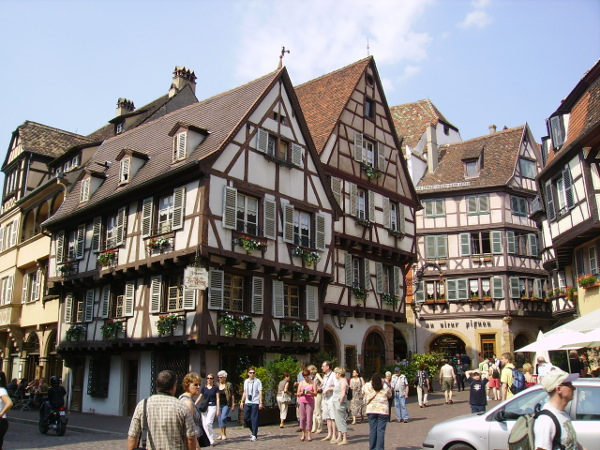
\includegraphics[scale=0.5]{images/architecturebretonne_wikipedia.jpg}
\caption{Éléments d'architecture bretonne typique du Sud de la France. (\href{http://commons.wikimedia.org/wiki/File:Colmar_-_Alsace.jpg}{Wikipédia.fr} CC-By-Sa)}
\end{figure}

\end{frame}



\end{document}
